\chapter{Конструкторский раздел}
\label{cha:design}

В данном разделе будет приведено описание схем алгоритмов
и вычислены их трудоемкости.

\section{Разработка алгоритмов}

На рисунках показаны схемы алгоритмов умножения матриц, стандартный и алгоритм Винограда.


\pagebreak
\subsection{Схема стандартного алгоритма умножения матриц}

\begin{figure}[h]
    \centering
    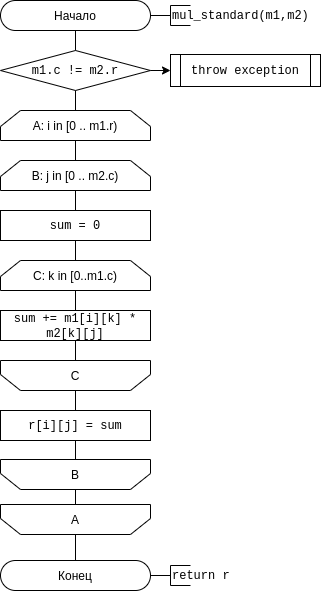
\includegraphics[width=0.6\textwidth]{2/inc/d1.png}
    \caption{Схема стандартного алгоритма умножения матриц}
    \label{fig:2.1}
\end{figure}


\newpage
\subsection{Схема алгоритма Винограда}

\begin{figure}[h!]
    \centering
    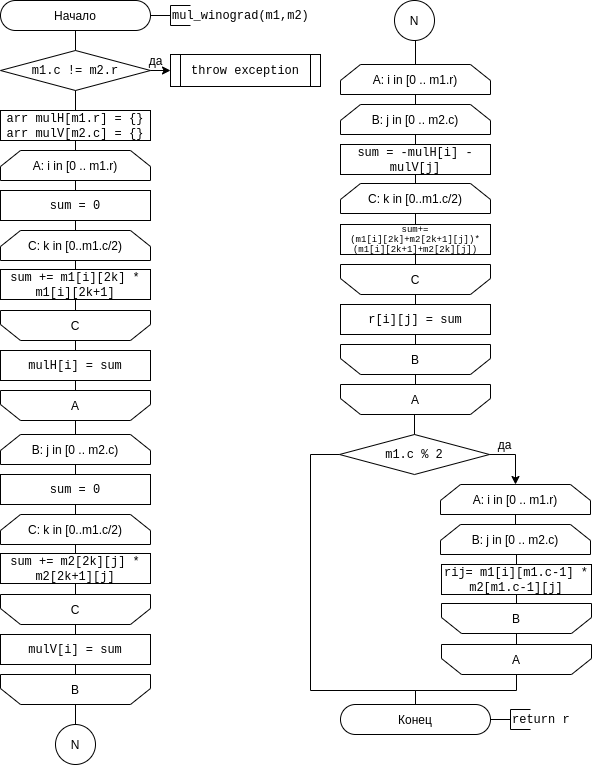
\includegraphics[width=1\textwidth]{2/inc/d2.png}
    \caption{Схема алгоритма Винограда}
    \label{fig:2.2}
\end{figure}

\begin{figure}[h!]
    \centering
    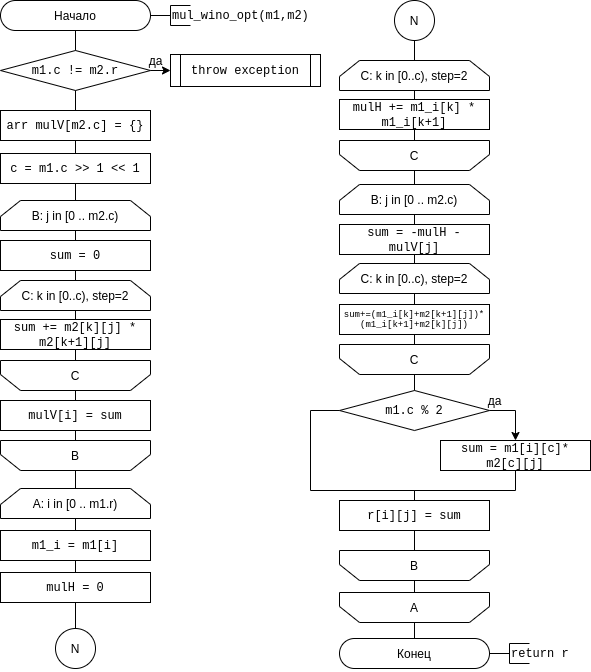
\includegraphics[width=1\textwidth]{2/inc/d3.png}
    \caption{Схема оптимизированного алгоритма Винограда}
    \label{fig:2.2}
\end{figure}

\clearpage
\section{Оценка трудоемкости}

Примечание: две матрицы можно перемножать $[l,m] * [m,n]$.


\subsection{Стандартный алгоритм}


\begin{tabular}{|c|c|}
    \hline
    $F_{bodyC}$ & $6$ \\\hline
    $F_{forC}$  & $2 + m (6 + 2) = 8m + 2$ \\\hline
    $F_{bodyB}$ & $8m + 6$ \\\hline
    $F_{forB}$  & $2 + n (8m + 6 + 2) = 8mn + 8n + 2$ \\\hline
    $F_{bodyA}$ & $8mn + 8n + 2$ \\\hline
    $F_{forA}$  & $2 + l (8mn + 8n + 2 + 2) = 8lmn + 8ln + 4l + 2$ \\\hline
    $F_{standard}$ & $8lmn + 8ln + 4l + 3$ \\\hline
\end{tabular}


\subsection{Алгоритм Винограда}

\begin{tabular}{|c|c|}
    \hline
    $F_{bodyC_1}$   & $9$ \\\hline
    $F_{forC_1}$    & $3 + m/2 \cdot (9 + 3) = 6m + 3$ \\\hline
    $F_{bodyA_1}$   & $6m + 6$ \\\hline
    $F_{forA_1}$    & $2 + l (6m + 6 + 2) = 6lm + 8l + 2$ \\\hline\hline
    $F_{bodyC_2}$   & $9$ \\\hline
    $F_{forC_2}$    & $3 + m/2 \cdot (9 + 3) = 6m + 3$ \\\hline
    $F_{bodyB_2}$   & $6m + 6$ \\\hline
    $F_{forB_2}$    & $2 + n (6m + 6 + 2) = 6mn + 8n + 2$ \\\hline\hline
    $F_{bodyC}$     & $18$ \\\hline
    $F_{forC}$      & $3 + m/2 \cdot (18 + 3) = 10.5m + 3$ \\\hline
    $F_{bodyB}$     & $10.5m + 11$ \\\hline
    $F_{forB}$      & $2 + n (10.5m + 11 + 2) = 10.5mn + 13n + 2$ \\\hline
    $F_{bodyA}$     & $10.5mn + 13n + 2$ \\\hline
    $F_{forA}$      & $2 + l (10.5mn + 13n + 2 + 2) = 10.5lmn + 13ln + 4l + 2$ \\\hline\hline
    $F_{if}$        & $\left\{
        \begin{array}{ll}
            1, \hspace{5.4cm} $л.с.$\\
            1 + 2 + l(2 + n(2 + 10)), \hspace{0.5cm} $х.с.$\\
        \end{array}
        \right.$ \\\hline\hline
    $F_{winograd}$  & $10.5lmn + 6lm + 6mn +\left\{
        \begin{array}{ll}
            13ln, \hspace{0.5cm} $л.с.$\\
            25ln, \hspace{0.5cm} $х.с.$\\
        \end{array}
        \right. + ...$ \\\hline
\end{tabular}


\subsection{Оптимизированный алгоритм Винограда}

\begin{tabular}{|c|c|}
    \hline
    $F_{bodyC_1}$   & $7$ \\\hline
    $F_{forC_1}$    & $2 + m/2 \cdot (7 + 2) = 4.5m + 2$ \\\hline
    $F_{bodyB_1}$   & $4.5m + 5$ \\\hline
    $F_{forB_1}$    & $2 + n (4.5m + 5 + 2) = 4.5mn + 7l + 2$ \\\hline\hline
    $F_{bodyC_2}$   & $5$ \\\hline
    $F_{forC_2}$    & $2 + m/2 \cdot (5 + 2) = 3.5m + 2$ \\\hline
    $F_{bodyC_3}$   & $12$ \\\hline
    $F_{forC_3}$    & $2 + m/2 \cdot (12 + 2) = 7m + 2$ \\\hline
    $F_{bodyB_3}$   & $\left\{
        \begin{array}{ll}
            7m + 10, \hspace{0.5cm} $л.с.$\\
            7m + 16, \hspace{0.5cm} $х.с.$\\
        \end{array}
        \right.$ \\\hline
    $F_{forB_3}$    & $\left\{
        \begin{array}{ll}
            2 + n(7m + 12), \hspace{0.5cm} $л.с.$\\
            2 + n(7m + 18), \hspace{0.5cm} $х.с.$\\
        \end{array}
        \right.$ \\\hline
    $F_{bodyA}$     & $\left\{
        \begin{array}{ll}
            7mn + 3.5m + 12n + 7, \hspace{0.5cm} $л.с.$\\
            7mn + 3.5m + 18n + 7, \hspace{0.5cm} $х.с.$\\
        \end{array}
        \right.$ \\\hline
    $F_{forA}$      & $\left\{
        \begin{array}{ll}
            2 + l(7mn + 3.5m + 12n + 7), \hspace{0.5cm} $л.с.$\\
            2 + l(7mn + 3.5m + 18n + 7), \hspace{0.5cm} $х.с.$\\
        \end{array}
        \right.$ \\\hline\hline
    $F_{wino_opt}$  & $ 7lmn + 3.5lm + 4.5mn +\left\{
        \begin{array}{ll}
            12ln, \hspace{0.5cm} $л.с.$\\
            18ln, \hspace{0.5cm} $х.с.$\\
        \end{array}
        \right. +...$ \\\hline
\end{tabular}


\section{Вывод}
В данном разделе было приведено описание схем алгоритмов и вычислены их трудоемкости.
Трудоемкости алгоритмов соответственно 8, 10.5, 7 (lmn - куб).
